This thesis tackled the challenge of accelerating Graph Neural Network inference by leveraging High-Level Synthesis techniques targeting FPGAs.

An HLS-based toolchain was designed to obtain a GNN inference accelerator starting directly from PyTorch.
PyTorch stands as one of the foremost high-level frameworks for neural network implementation, extensively recognized and employed within the community, making the proposed toolchain suitable for different applications.

The results of this research significantly contribute to the field of GNN acceleration, introducing a new perspective about how it is possible to obtain hardware accelerators for GNNs even without having any hardware design knowledge.
The toolchain offers different possibilities and provides various optimization passes that can be used to fine-tune the accelerator capabilities.

Within the spectrum of optimizations made available by this toolchain, this thesis primarily delved into two key techniques: the loop unrolling technique in SODA-OPT and the parallel memory access of PandA-Bambu with an external memory of thirty-two channels.
These optimizations allowed to achieve encouraging and promising results in accelerating the inference of the GCN model analyzed.
By studying and understanding the model bottlenecks, it is possible to achieve consistent improvements.

Lastly, this study has also made substantial contribution in enhancing Torch-MLIR\@.
A new feature, the support of the constant of Tuple type, has been added and different areas of improvement have been identified, where more work would be needed to implement functionalities for the complete support of PyTorch Geometric.
Before this research, no examples were available on how to use Torch-MLIR with Graph Neural Networks, and the compatibility of PyTorch Geometric and Torch-MLIR was still an unexplored area.

\section{Future developments}
\label{sec:future-dev}%

\begin{figure}[t]
    \centering
    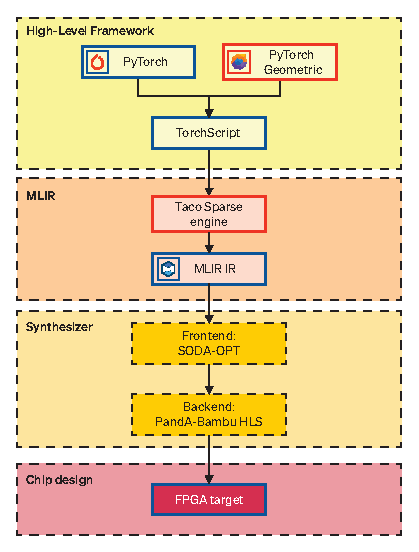
\includegraphics[height=0.5\textwidth]{Images/toolchain_future}
    \caption{Future FPGA Toolchain for Graph Neural Network Acceleration}
    \label{fig:toolchain-future}
\end{figure}

This thesis represents a significant advancement in the field of GNN acceleration.
Nonetheless, there exist opportunities for further enhancement through the implementation of novel features.

Primarily, future works could build upon the innovative contributions of this thesis in terms of enhancing compatibility between PyTorch Geometric and Torch-MLIR\@.
PyTorch Geometric offers valuable features and pre-established classes for implementing Graph Neural Networks.
Integrating this advanced framework into the toolchain would mark another significant step forward.
This thesis identified the needed area of improvement, representing a possible starting point for these future works.

Another improvement that can be applied to the presented toolchain is the support of sparse tensors.
At the actual state, Torch-MLIR is not capable of lowering PyTorch sparse tensors to the Linalg dialect, even if it already supports them.
For this reason, some work would be needed on Torch-MLIR to implement this feature, possibly using PyTaco, which would bring a significant advantage also in the resulting accelerators, having the possibility to exploit faster computation with sparse tensors.
An additional enhancement that can be integrated into the proposed toolchain involves extending support to sparse tensors.
Currently, Torch-MLIR cannot convert PyTorch sparse tensors into the Linalg dialect, even if MLIR~\cite{9370308} already has a way to represent them~\cite{Bik_2022}.
Consequently, implementing this feature in Torch-MLIR would require dedicated efforts, producing substantial benefits in the toolchain resultant accelerators.
Even if the resulting accelerators, as discussed in Chapter~\ref{ch:chapter_six}, greatly increase performance and reduce the computational time, this enhancement would enable leveraging faster computations through the use of sparse tensors by further improving the performance of the accelerator.

Figure~\ref{fig:toolchain-future} shows how the toolchain could appear with the implementation of the above-mentioned future developments.
In particular, PyTorch Geometric would be part of the supported high-level frameworks, and the engine used by PyTaco to annotate sparse tensors would be adapted and used to convert the TorchScript representation of the model into MLIR with sparse tensor dialect, ready to be received as input by SODA-OPT\@.

In conclusion, ongoing support and dedicated efforts are consistently aimed at advancing SODA-OPT~\cite{9786533} and PandA-Bambu~\cite{9586110} through the integration of novel functionalities.
The continuous evolution of these tools represents an alternative way of progress over that the classic hardware design techniques, as the introduction of fresh SODA-OPT passes and PandA-Bambu optimizations have the potential to open novel opportunities for refining and optimizing the synthesized hardware accelerators.